\chapter{Background}
\lhead{\emph{Background}} 
\label{chap:background}	

The goal of machine learning is to avoid solving a specific task by explicitly programming an algorithm. In order to do this, machine learning tries to optimise a performance criterion using example data or past experience. When trying to solve a new task, it might be difficult to design a complete specification of the algorithm behaviour while it might be possible to obtain samples of the expected behaviour or to get feedback on the quality of the behaviour. Machine learning models can be predictive, i.e. make predictions based on new data, or descriptive, when the task of the model is to gain knowledge from data, or both \cite{alpaydin_introduction_2010}.

Reinforcement learning can be loosely related to how we as humans, learn to interact with our environment. For most of our life we do not have access to an explicit teacher, but we do have access to a direct sensorimotor connection to our environment providing feedback. Leveraging this feedback offers an indication about the consequences of an interaction with the environment. This indication can help us determine what to do to achieve a certain outcome. Reinforcement learning is the machine learning approach for learning goal oriented tasks from interaction.

Other approaches to machine learning include \textit{supervised learning} and \textit{unsupervised learning}. In supervised learning, a set of labelled examples provided by an external entity is used for the learning. Although supervised learning has been shown to be highly efficient for certain problems, obtaining the input-output pairs in an interactive problem can be extremely difficult. Indeed, the pairs should be representative of the expected behaviour as well as of all the states in which the agent should act. On the other hand, unsupervised learning finds hidden relationships between unlabelled inputs. Despite reinforcement learning having no direct access to the input-output examples, it should be considered a paradigm in its own right and not a kind of unsupervised learning. Indeed, it tries to maximise a reward signal instead of finding hidden pattern in the inputs.

Instead of relying on an oracle to instruct a learner the best action to take, reinforcement learning has to rely on a signal related to the quality of its decision \cite[p.~25]{sutton_reinforcement_1998}. The signal, which indicates what to do, but not how to do it, is expressed by a sanction called a \textit{reward} \cite[p.~18]{yves_glorennec_reinforcement_2001}. The reward can be positive, negative or neutral. It might be influenced by the taken action as well as the agent's past actions (delayed impact). The goal of reinforcement learning is thus to optimise a reward function by interacting with its environment (i.e. taking actions) and observing the resulting reward \cite{g._barto_1_2008}. Actions which have a positive outcome or avoid negative one will be preferred (reinforced). This is why reinforcement learning can be seen as a trial and error search.

% - learning agent must have access to: information about the current state, mean to affect the environment through interaction, and an indication about the quality of the interaction

% - RL is a sort of trial and error search
% - Use training information which evaluates action rather than instructs by giving correct action [RLNA p.25]
% - require reward, i.e. indication of the quality of interaction, because no oracle exists
% - Oracle could indicate which is the best action to take in this situation.
% - can see reward as a sanction (positive, neg or neutral) [RLAO p18] which indicates what to do but not how to do it
 
% - Must be able to take into account the fact that an action might have a direct or indirect (delayed) impact on following reward
% - optimizing an unknown reward function without direct access to the function but with the ability of taking actions observing the resulting reward. [Reinforcement learning and its relationship with supervise learning Andrew G barot]
% - agent needs to balance between exploration and exploitation to avoid getting stuck in local optima [EDMALAS Tuyls]

% - Action which have a positive return will be favoured over time, i.e the benefice behaviour will be reinforced. 
% => trade -off of exploration and exploitation.

\section{Markov Decision Processes}

In reinforcement learning, it is important to make the distinction between an agent and the environment. An agent is a computational mechanism able to learn and to take actions based on external information \cite{panait_cooperative_2005}. The environment is everything else. More precisely, it is everything which cannot directly be modified by the agent \cite[p.~50]{sutton_reinforcement_1998}.

\begin{figure}
\centering
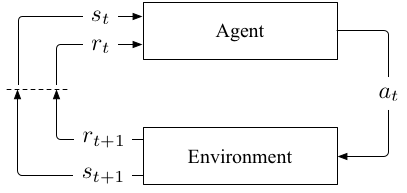
\includegraphics[width=0.5\textwidth]{imgs/rl-env.png}
\caption[The agent-environment interactions in a Markov decision process]{The agent-environment interactions in a Markov decision process \protect\footnotemark.}
\label{fig:agent-env-interaction}
\end{figure}


\footnotetext{Figure taken from \cite{sutton_reinforcement_1998}.}


The interaction between an agent and the environment is done at discrete time-steps. At each time-step, the agent observes the environment and takes an action accordingly. The environment will then transition to another state and provide a numerical signal, the reward, related to the transition. When a single agent is present in the environment, Markov decision processes (MDPs) can be leveraged to express mathematically the reinforcement learning problem \cite{puterman_markov_1995}. The interaction of the agent with the environment as depicted in fig.~\ref{fig:agent-env-interaction} creates a sequence of tuples $(s_t, a_t, r_t, s_{t+1})$ describing one \textit{trajectory} or \textit{episode}. Besides a finite set of states and actions, $S$ and $A$, the MDP requires a definition of its dynamics. The dynamics of any MDP can be defined by the probability to move to state $s' \in S$ and receive reward $r \in \realnumbers$ by taking action $a \in A$ in state $s \in S$.

$$p(s', r | s, a) = P(s_{t}=s', r_{t}=r \mid s_{t-1}=s, a_{t-1}=a)$$

Based on the recorded trajectory, it is possible to calculate the return or the sum of reward from time $t$ to the end of the episode.

$$G_t=\sum_{k=0}^{T} \gamma^{k} r_{t+k+1} = r_{t+1} + \gamma G_{t+1} \text{ with } G_T=0$$

Because an episode can be infinite (continuing task) or finite (episodic task), a discounting factor $\gamma$ is introduced in the formulation to avoid unbounded sums. The discount factor also determines the importance of future reward compared to immediate reward. 

When interacting with the environment, an agent is expected to choose an action $a_t$ in state $s_t$ according to a certain policy $a_t = \pi(s_t)$. If the agent follows a fixed policy, it is possible to express the expected return using the \textit{state-value function}. The function expresses the amount of reward an agent can expect to receive when starting in state $s$ and following $\pi$

$$v_{\pi}(s) = \E_{\pi}[G_t|S_t=s]$$.

Similarly, the expected return by taking action in state $s$ and then following $\pi$ is expressed by the \textit{action-value function}, 

$$q_{\pi}(s,a) = \E_{\pi}[G_t|S_t=s, A_t=a]$$.

Both functions can be used to organise and structure the search for good policies \cite[p.~73]{sutton_reinforcement_1998} and can be calculated iteratively using the Bellman equation \cite{bellman_dynamic_2003}. The Bellman equation expresses the relationship between the value of a state and the value of its successor state. Moreover when the MDP is finite, the Bellman equation for the optimal state-value function $v^*$ has a unique solution independent of the policy $\pi$. When $v^*$ is available, it is straight forward to define an optimal policy $\pi^*$ by being greedy with respect to the state-value function. 

\begin{equation}\label{eq:v_greedy}
v^{\pi^*}(s) = \max_{\pi} v^{\pi}(s) \text{ for } \forall s \in S
\end{equation}

% If the optimal action-value function $q^*(s,a)$ is available, the necessary lookahead and can directly choose action maximizing the q(s,a) [RLAN p.64]

When a complete description of the underlying MDP is available, an optimal policy can be determined without experiencing the environment linked to it. In such cases, \textit{model-based} methods can be used. An example is dynamic programming. More often though, the dynamics of the environment might not be known and must be learned by interacting with the MDP. Such techniques are called \textit{model-free}.

% # Mathematical Framework
 
% ## Base theory
 
% - When single agent is interacting with the environment, can use classic formalization of sequential decision making where actions influence all (RLAN p47 + REF TO MDP)
% - Idealization of the reinforcement learning problem (Puterman 1994)
 
% - Agent = learner, everything else is the environment [RLAN p.49]
% - Agent is a computational mechanism that exibits degree pf autonomy, perfomring actions based on information [CMAL Liviu]
% - Interaction is done using a discrimination of time => sequence of tuple (St, At, Rt, St+1) (sequence is called an episode)
% - dynamics of MDP, i.e. how we can move around is defined by $p(s', r | s,a)$
% => LOOKUP [EDOMALAS Tuyls] for introduction
% => LOOKUP [DRLORB Leottau] for introduction
% - characterize environment dynamics [RLAN p.48]
% - The environment give rise to the reward signal
 
% => Picture
 
% - Learner use reward as a description of its goal. Always learns to maximize it. Must be carefully crafted to avoid the learner to learn only sub task and not the global one. 
% - A learning agent in state $s_t$ is expected to choose an action $a_t$ according to a certain policy $a_t = \pi(s)$
% - Judge quality of policy by the expectation of future reward expressed by value functions
% - $G_t=\sum_{k=0}^{T} \gamma^{k}R_{t+k+1} = R_{t+1} + \gamma G_{t+1}$ with $G_T=0$ [RLAN p.55 + REF BASE]
% - Discounting is used to avoid exploding reward 
% - Discount rate determines importance of future reward compared to immediate reward 
% - When episode terminates => call episodic task : can assume independence btwn episode, when episode doesn't terminate => continuing task [REF]
 
% - Two main value-function are used which can be estimated through experience [RLAN p.58]
% - State Value function $v_{\pi}(s) = \E_{\pi}[G_t|S_t=s]}$, expected return when starting in s and following $\pi$. It indicates how good the state $s$ is. 
% - Action Value function $q_{\pi}(s,a) = \E_{\pi}[G_t|S_t=s, A_t=a]$ = expected return by taking action $a$ and then following $\pi$ 
% - Use value functions to organize and structure the search for good policies [RLAN p.73]
 
% - Goal: for every initial state, find a an optimal policy, i.e. a policy which maximize the expected return, i.e the long term reward that the agent might be able to accumulate over time. [RLAO p 20]
 
% - an optimal an optimal policy $\pi^*$ is defined by $v^*(s) = \max_{\pi} v_{\pi}(s)$ or equivalently defined by the optimal action value function $q^*(s, a)$.
% - One can show that $v_{\pi}(s)$ and $q_{\pi}(s,a)$ both can be expressed in the form of a Bellman equation [REF]
 
 % - When a complete description of environment is available (access to the transition probability), model-based technics (such as DP) can be used to find an optimal an optimal policy $\pi^*$ without having to experience the MDP
 % - Otherwise, as in most cases the dynamics of the environment are not known and must be learned by interacting with the MDP, such techniques are called model-free.
 
% - If state, i.e the information given to the learner contains all the information that make a difference for the future, the Markov property holds. In a Markov decision process, the probability of each state and reward depend only on the immediately preceding state and action. thus the state must have all necessary information that make a difference for the future. [Altman, Eitan (1999).]
 
 % - MDP considered solved when an optimal policy has been found, i.e $v*(s) = \max_{\pi} v_{\pi}(s)$
% - Using Bellman optimality https://www.sharelatex.com/project/5ae9981d73c6b024e0c990c8equation [REF] we can assume that the value of a state under an optimal policy must equal the expected return for the best action from that state
% - Any policy which is greedy in term of $v_{*}$ will be an optimal policy
% - If $q^*(s,a)$ is available, don't need the look ahead and can directly choose action maximizing the q(s,a) [RLAN p.64]
 
Using the reward as a description of its goal, the objective of the agent is to find an optimal policy $\pi^*$ which maximises the long term reward that it might be able to accumulate over time \cite{yves_glorennec_reinforcement_2001}.

\subsection{Learning with complete knowledge of the environment}
\label{sec:complete_knowledge}
 
In model-based learning, two main approaches can be used to find an optimal policy. The policy can be directly manipulated with the \textit{policy iteration} method. An other approach is \textit{value iteration}, which looks for the optimal value function \cite{yves_glorennec_reinforcement_2001}.

The idea behind policy iteration and value iteration is to ask what happens if, after computing $v_{\pi}(s)$, instead of selecting $a=\pi(s)$ in $s$, another action is selected. This is embodied by the action-value function $q(s,a)$. Generalising this idea to all states, a new policy can be computed using

\begin{equation}
\label{eq:policy_improvement}
 \pi'(s) = \argmax_a q_{\pi}(s, a)
\end{equation}.

Using the \textit{policy improvement theorem} \cite[p.~78]{sutton_reinforcement_1998}, the new policy $\pi'(s)$ must be better or equal to the initial one, i.e.

 $$q_{\pi}(s, \pi'(s)) = v_{\pi'}(s) \geq v_{\pi}(s) = q_{\pi}(s, \pi(s))$$. 
 
Following now $\pi'$ instead of the initial policy should give rise to higher or equal return for all states s. Making a new policy that improves on the original one by making it greedy with respect to the value function of the original as in equation~\ref{eq:policy_improvement} is called \textit{policy improvement}. The combination of the determination of the value-function with respect to $\pi$ (\textit{policy evaluation}) with policy improvement, is called policy iteration method (alg.~\ref{alg:policy-iteration}). 

\begin{algorithm}[H]
\caption{Policy Iteration \cite{sutton_reinforcement_1998}}
\label{alg:policy-iteration}
\begin{algorithmic}
\\
\BState \textbf{\emph{Initialisation}}:
	\State $V(s) \in \realnumbers \textrm{ and } \pi(s) \in A \textrm{ arbitrarily for all } s \in S$
\\
\BState \textbf{\emph{Policy Evaluation}}:
	\Repeat
		\State $\Delta \gets 0$
		\ForAll{$s \in S$}
			\State $v \gets V(s)$
 \State $V(s) \gets \sum_{s', r} p(s', r \mid s,\pi(s)[r + \gamma V(s')]$
			\State $\Delta \gets \max(\Delta, \mid v - V(s)\mid)$
		\EndFor
 \Until{$\Delta < \Theta$}
\\
\BState \textbf{\emph{Policy Improvement}}:
 \State $\textit{policy-stable}\gets \textit{true}$
 \ForAll{$s \in S$}
 \State $\textit{old-action}\gets \pi(s)$
 \State $\pi(s) \gets \argmax_a \sum_{s', r} p(s', r' \mid s,a)[r + \gamma V(s')]$
 \If {$\textit{old-action} \neq \pi(s)$}
 $\textit{policy-stable}\gets \textit{false}$
 \EndIf
 \EndFor

 \If {$\textit{policy-stable}$}
 \State \textbf{return} $V \approx v^*, \pi \approx \pi^*$ 
 \Else
 \State \textbf{goto} \emph{Policy Evaluation}.
 \EndIf
\end{algorithmic}
\end{algorithm}


By contrast, value iteration (alg.~\ref{alg:value-iteration}) combines in a single update one sweep of policy evaluation and one sweep of policy improvement. It does so by avoiding the tracking of the policy and concentrating on finding the optimal value function. When the optimal value function is found, a deterministic policy can be found using the greedy approach as in eq.~\ref{eq:v_greedy}.

\begin{algorithm}[H]
\caption{Value Iteration \cite{sutton_reinforcement_1998}}
\label{alg:value-iteration}
\begin{algorithmic}
\\
\State $\Theta > 0$
\State Initialise $V(s)$, for all $s \in S^+$, $a \in A(s)$, arbitrarily except that $V(terminal) = 0$
\\
\Repeat
	\State $\Delta \gets 0$
	\ForAll{$s \in S$}
		\State $v \gets V(s)$
		\State $V(s) \gets \max_a \sum_{s', r} p(s', r \mid s,a)[r + \gamma V(s')]$
\State $\Delta \gets \max(\Delta, \mid v - V(s)\mid)$
\EndFor
\Until{$\Delta < \Theta$}
\\
Output a deterministic policy, $\pi \approx \pi^*$, such that\\
$\pi(s) = \argmax_a \sum_{s',r} p(s', r \mid s, a)[r + \gamma V(s')] $
\end{algorithmic}
\end{algorithm}
Both methods can be seen as a version of \textit{Generalised Policy Iteration}. In Generalised Policy Iteration two processes interact. One which makes the value function consistent with the current policy, and the other which makes the policy greedy with respect to the current value function \cite[p.~86]{sutton_reinforcement_1998}. 

% - When policy is fixed, Optimal value function can be estimated using iterative solutions relying on the bellman equation , this step is called policy evaluation.

% $v^*(s) = \max_a \sum_{s'}p(s',r | s,a)[r + \gammav*(s')]$
 
% - Can rely on the Policy improvement theorem which says that if $q_{\pi}(s, \pi'(s)) \geq v_{\pi}(s)$, then $v_{\pi'} \geq v_{\pi}$. The process of making a new policy that improve on an original policy , by making it greedy with respect to the value function of the original policy is called policy improvement [RLAI 79]

% %https://stackoverflow.com/questions/37370015/what-is-the-difference-between-value-iteration-and-policy-iteration
% %https://www.quora.com/How-is-policy-iteration-different-from-value-iteration
 
% - Policy iteration
% - Start from a initial policy (can be random) and improve it iteratively
% - policy evaluation followed by policy improvement until convergence.
% - two interacting process, one making the value function consistent with the current policy (policy evaluation) and the other making the policy greedy with respect to the current value function (policy improvement). [RLNA p.86]
 
% - Value iteration
% - Avoids the policy evaluation step of Policy iteration by stopping after a single sweep (one update of each state)
% - Find optimal value function directly and extract a single time the policy from it (don't track it during learning)

\subsection{Learning with incomplete knowledge of the environment} 

When value functions need to be estimated using experience only, two main \textit{model-free} approaches exist. The first one relies on Monte-Carlo experiments using sampled episodes, while the second one can learn directly from raw experience. Both approaches can be used to find optimal policies without any information beside experience \cite[p.~98]{sutton_reinforcement_1998}.

The first approach is encompassed by Monte-Carlo Methods. They first generate experience (i.e episodes) by following a policy $\pi$ and recording the resulting sequence of tuples $(s_t, a_t , r_t)$. The main idea behind the Monte-Carlo approach is to estimate the state-value function based on the average return $G_t$ observed after visiting that state. 

$$V(s_t) \longleftarrow V(s_t) + \alpha[G_t - V(S_t)]$$ 

This means that instead of computing the value of each state by using the model of the MDP, it relies on the empirical average return starting in that specific state \cite[p.~115]{sutton_reinforcement_1998}. Monte-Carlo methods are not bootstrapped which means they do not build the estimate for each state based on other estimate. With those methods, the full sequence of received rewards is known in advance. Therefore, it is possible to know the long term return from a specific state. Without access to the model of the MDP, the value for each action in a specific state must be estimated. Unlike for model-based methods, the single step look-ahead used to determine the best action cannot be made \cite[p.~96]{sutton_reinforcement_1998}. 

When experiencing the environment, choosing which action to take in a certain state can have a big impact on the learning process. Indeed, an agent can either exploit his knowledge and take actions that will yield high reward in the short term or take a sub-optimal route now, with the hope of achieving better results in the future. This is called the \textit{exploration and exploitation trade-off}. 
Finding the right balance between the two has been shown to be problematic \cite{sutton_reinforcement_1998, bloembergen_evolutionary_2015}. To be certain of the convergence of the Monte-Carlo methods, all actions in each state must be selected with a non zero probability to ensure constant exploration of the state space and all state transition \cite[p.~97]{sutton_reinforcement_1998}. 

There are two ways to find an optimal policy and ensure the exploration. Either by \textit{on-policy learning}, where the policy used to make the decisions is evaluated and also improved, or by \textit{off-policy learning}, where a different policy than the one used to generate the data is evaluated and improved.

With on-policy learning, the agent commits to always exploring by making the followed policy soft, i.e. $\pi(a|s) > 0$ $\forall s \in S$, $\forall a \in A$, but gradually shifting closer to a deterministic policy \cite[p.~100]{sutton_reinforcement_1998}. An example of such a policy is the $\epsilon$-\textit{greedy} one, where the greedy action is selected with a probability $1 - \epsilon$, while the rest of the time a random action is selected. By contrast, off-policy learning uses two different policies. One policy that is learned about and that becomes the optimal one and one for exploring. 

% The other one is more exploratory and used to generate behaviour (target versus behaviour policies) \cite[p.~103]{sutton_reinforcement_1998}. This means that the agent learns a deterministic optimal policy that may be unrelated to the exploring policy followed \cite[p.~115]{sutton_reinforcement_1998}. 

% Policy iteration and value iteration can be used to estimate an optimal policy in both cases.

% ### Monte-Carlo
% - Goal is to estimate the value function without complete knowledge of environment, i.e learn from experience
% - Value function are estimated using the final reward, not based on the estimations of neighboring states
% - requires only experience not need for knowledge of underlying model dynamics 
% - Generate experience by following policy $\pi$ (episode(s)) (record sequence of tuple (S, A , R), Sample episode
% - Monte-Carlo methods can be used to find optimal policies given only sample episodes and no information about environment [RLAN p98]
 
% - based on averaging sample returns for each state-action pair. Compared to bandit problems, the return after taking an action in one step might influence the later states. [RLAN p91] 
 
% - Main Idea : estimate the state value bases on the average return observed after visiting that state, i.e instead of computing the value of each state by using a model of the dynamics, rely on average return that start in that state [RLAN 115]
% - Easy to determine policy if rely on action-value function to build an optimal greedy policy. $\pi(s) = \max_a q(s,a)$
% - The estimate for each state are independent because not build up on the estimate of any other state => No bootstrapping
 
% - Must estimate action values, q(s,a) as we can't rely on the state values alone to determine a policy. (Model Free). => if know model, can look one step ahead choose action leading to best combination of reward and next state => Must estimate the value for each action [RLAN 96]
 
 % - To improve the estimation to the action values, we can't rely on a deterministic policy to move along the MDP => 
 % - require to explore to encounter each state action pair because exploitation is good for short term but not for long. 
 % => Non zero probability of selecting all actions in each state. [RLAN p.97]
 % => By doing so ensure constant exploration of the state space and state transition. 
 
 % - Both Policy Iteration and Value iteration can be used to estimate an optimal policy
 % - both the estimate of the value function and the policy are improved at the same time (i.e policy evaluation followed by policy improvement) where policy improvement is done by making the policy greedy with respect to the current value function.
 % - Still need to make sure that the policy used to experience the MDP still explores, i.e all actions are selected infinitely often
 
 % - on-policy = evaluate and improve the policy which is used to make decision
 % - Compromise : Lear action value for an near-optimal policy
 % - Make policy soft, ie.e $\pi(a|s) > 0$ for all a and s but gradually shifted closer to a deterministic policy [RLAN p.100]
 % - agent commits to always exploring and tries to find the best policy
 % - example e-greedy
% - converge toward the optimal policy while keeping a non zero proba => convergence ensured by the policy improvement theorem [REF]
 
% - off-policy = evaluate a different policy than the one used to generate the data
% - Most straight forward : use one policy that is learned about and that becomes the optimal one, while the other one is more exploratory and used to generate behaviour. (target vs behaviour policies) [RLNA p.103]
 % - agent explores but learns a deterministic optimal policy that may be unrelated to the exploring policy followed [RLNA 115]
% - Can be used to learn from external source acting as the behavioural agent

% - Can be implemented incrementally on an episode by episode basis [ RLAN 108], 
% - (Risk for off-policy: Learns from tail of episodes when all remaining actions in the episode are greedy -> use TD [RLAN p 111])

In place of waiting the end of an episode to know $G_t$, it is possible to update an estimate based on another learned estimate, i.e. bootstrap. This is call \textit{temporal difference} (TD) learning. Instead of using the Monte-Carlo methods update, TD methods change the update rule to 
 
 $$V(s_t) \longleftarrow V(s_t) + \alpha[R_t +\gamma(V(s_t+1) - V(s_t)]$$. 
 
Both update methods follow the canonical form $$\text{new-estimate} \longleftarrow \text{old-estimate} + \text{step-size} \times [ \text{target} - \text{old-estimate}]$$ where it is assumed that the target indicates a desirable direction in which to move \cite[p.~30]{sutton_reinforcement_1998}.
 
There is no need to wait until the end of an episode to know the update of $V(s_t)$ by using the second update rule. Only the next time step is required by $TD$ methods. The $[R_t +\gamma(V(s_t+1) - V(s_t)]$ part of the update can be seen as an error (\textit{$TD$ error}) which measures the difference between the estimated value of $s_t$ and the better estimate $R_t +\gamma(V(s_t+1)$ \cite[p.~121]{sutton_reinforcement_1998}. It can be implemented online in a fully incremental fashion \cite[p.~124]{sutton_reinforcement_1998}. If the update is made after every transition, the method is called \textit{TD(0)}. It has been proven that by following a fixed policy $\pi$, $TD(0)$ will converge to $v_{\pi}$, if the learning gain $\alpha$ decreases sufficiently slowly towards zero \cite{sutton_learning_1988}. A comparison between Monte-Carlo and $TD$ methods can be found in \cite[p.~123]{sutton_reinforcement_1998}.

By following the pattern of generalised policy iterations, it is possible to determine an optimal policy. Just like for Monte-Carlo methods, the trade-off between exploration and exploitation can be approached from two different angles.

The action-value function $q_{\pi}(s, a)$, rather than the state-value function, is estimated using 
 
 $$Q(s_t, a_t) \longleftarrow Q(s_t, a_t) + \alpha[r_{t+1} + \gamma Q(s_{t+1}, a_{t+1}) - Q(s_t, a_t)]$$
 
 which can be executed after every transition. This update method is the base for the on-policy \textit{Sarsa} control algorithm. Sarsa converges to an optimal policy and an optimal action-value function as long as the policy converges at the limit to a greedy policy. This can be achieved by using an $\epsilon$-greedy policy where $\epsilon = 1/t$ \cite[p.~129]{sutton_reinforcement_1998}. The Sarsa algorithm is an on-policy method because the action selection is done relative to the same policy as the one that is improved. The pseudo-code for the algorithm can be found in alg.~\ref{alg:sarsa}. 
 
\begin{algorithm}[H]
\caption{Sarsa (on-policy TD control) \cite{sutton_reinforcement_1998}}
\label{alg:sarsa}
\begin{algorithmic}
\\
\State $\alpha \in (0,1], \epsilon > 0$
\State Initialise $Q(s,a)$, for all $s \in S$, $a \in A(s)$, arbitrarily except that $Q(terminal, \cdot) = 0$
\\
\ForAll{episodes}
	\State Initialise $S$
 \State Choose $a_t$ using policy derived from Q (e.g., $\epsilon$-greedy)
 \ForAll{steps in episode}
 \State Take action $a_t$, observe $_t$ and $s_{t+1}$
 \State Choose $a_{t+1}$ using policy derived from Q (e.g., $\epsilon$-greedy)
 \State $Q(s_t,a_t) \gets Q(s_t,a_t) + \alpha[r_t + \gamma Q(s_{t+1}, a_{t+1}) - Q(s_t,a_t)]$,
 \State $s_t \gets s_{t+1})$, $a_{t} \gets a_{t+1}$
 
 \If {$s_t$ is terminal}
 \State \textbf{return}
 \EndIf
 \EndFor
\EndFor
\end{algorithmic}
\end{algorithm}

Watkins and Dayan presented another approach called \textit{Q-Learning} \cite{watkins_q-learning_1992}. Q-Learning directly approximates the optimal action-value function independently of the policy being followed. For convergence to be guaranteed, the followed policy must enable all state-action pairs to be updated.

 $$Q(s_t, a_t) \longleftarrow Q(s_t, a_t) + \alpha[r_t + \max_a Q(s_{t+1}, a_{t+1}) - Q(s_t, a_t)]$$

Q-learning is an off-policy control method because the action selection is taken with respect to an $\epsilon$-greedy algorithm while the action value function update is determined using a different policy i.e. one that is directly greedy with respect to the action value function (indicated by $\max_a Q(s_{t+1}, a_{t+1})$). 


\begin{algorithm}[H]
\caption{Q-learning (off-policy TD control) \cite{sutton_reinforcement_1998}}
\label{alg:q-learning}
\begin{algorithmic}
\\
\State $\alpha \in (0,1], \epsilon > 0$
\State Initialise $Q(s,a)$, for all $s \in S$, $a \in A(s)$, arbitrarily except that $Q(terminal, \cdot) = 0$
\\
\ForAll{episodes}
 \State Initialise $S$
 \State Choose $a_t$ using policy derived from Q (e.g., $\epsilon$-greedy)
 \ForAll{steps in episode}
 \State Take action $a_t$, observe $r_t$ and $s_{t+1}$
 \State $Q(s_t,a_t) \gets Q(s_t,a_t) + \alpha[r_t + \gamma \max_a Q(s_{t+1}, a) - Q(s_t,a_t)]$,
 \State $s_t \gets s_{t+1})$
 
 \If {$s_t$ is terminal}
 \State \textbf{return}
 \EndIf
 \EndFor
\EndFor
\end{algorithmic}
\end{algorithm}

Up to now all methods presented have been relying on estimating a value-function in order to find an optimal policy. Another approach is to learn directly a parameterized policy $\pi(a|s, \theta)$ which select actions without consulting any value function \cite[p.~323]{sutton_reinforcement_1998}. This kind of techniques are called \textit{policy gradient methods}. 

Learning the parameters of the policy is done via the gradient of some performance measure $J(\theta)$. To ensure convergence, it is required that the policy never becomes fully deterministic. This can be achieved by using parameterized numerical preferences for each state-action pair. An example of such parameterization is the softmax distribution. 

Methods which learn both an estimation of the policy and the value function are called \textit{actor-critic methods}.

% ### Temporal Difference
 % - Can learn directly from raw experience without model same as MC. 
 % - Instead of having to wait until end of episode to know $G_t$ as in MC, just wait next time step
 % - $V(s_t) <- V(s_t) + a*[G_t - V(S_t)]$ Change to $V(s_t) <- V(s_t) + a*[R_t +b(V(s_t+1) - V(s_t)]$
 % - bracket stuff can be seen as an error
 
 % - TD methods update their estimate in part on other estimates => bootstrap => can be implemented online, fully incremental fashion [RLAN 124]
 % - Can even be computed after every transition (TD(0))
 % - Proved that with fixed $\pi$ will converge to $v_{\pi}$ if learning gain a decreses sufficiently slowly twoards zero [RLNA 124 & Sutton RS Learning to predict by temporal difference 1989]
 
 % - interesting comparison between Monte-Carlo and TD can be seen in [RLA 123]
 
 % - Goal : Estimate action-value function $q_{\pi}(s, a)$
 % https://groups.google.com/forum/#!topic/rl-list/4Efnr0gXhAU
 % https://www.reddit.com/r/MachineLearning/comments/417wqu/on_policy_vs_off_policy_in_rl/
 % https://stats.stackexchange.com/questions/184657/what-is-the-difference-between-off-policy-and-on-policy-learning
 % https://www.researchgate.net/post/what_is_the_difference_between_value_iteration_and_policy_iteration_methods_in_reinforcement_learning
 
 % - On-Policy : $Q(St, At) \longleftarrow Q(St, At) + \alpha[Rt+1 + \gamma Q(St+1, At+1) - Q(St, At)]$ (SARSA) [RLAN 129 + REF]
 % - done after every transition
 % - convergence depends policy dependence on Q. Must make sur that all action-state pairs are visited but policy still converge to greedy policy (e-greedy with e=1/t)
 % - On-poliocy because action selection of at is done relative to the same policy i.e e-greedy
 
 % - Off-Policy : $Q(St, At) <- Q(St, At) + a[Rt + \max_a Q(St+1, At+1) - Q(St, At)]$ (Q-Learning) [RLAN 131] [Watkins and Dayan 1992]
 % - in this case directly approximate the q* independently of the policy being followed. just need to make sure all pair a updated. 
 % - Q-learning is an off-policy control method because the action selection is taken with respect to an ǫ-greedy algorithm while the action value function update is determined using a different policy i.e. one that is directly greedy with respect to the action value function.
 % => Update (greedy) and selection (e-greedy) are not based on same policy
 
 
% ### Policy gradients [RLAN 323 + REF]

 % - If rely on action-value, policy only exists because of it
 % - Policy gradient relies n a parameterized policy. $\pi(a|s, \theta)$
 % - learning parameters using some performance measure $J(\theta)$
 % - Update using gradient update rule
 % - Need to be differential with respect to parameters
 % - To insure convergence => need policy to never become deterministic during learning 
 % - parameterize using preference for each action pair, example softmax distribution.
 % => better than e-greedy because can approach deterministic while e-greedy has always a predefined proba
 
% EXTRA INFO 
% - Using the MDP can derive the expected reward for state-action pairs, i.e estimate a value function related to how good it is to be in that state and take action a
% - Thank-s to the Bellman Equation, a relation between the value of a state and the the value of the successor can be established
% - value off start start equal the value of the expected next state plus reward expected along the way.
% - If maintain estimate of long term reward of the action values, at least one if greatest => greedy action [RLNA p.26]
% - If select only greedy, exploitation, i.e. maximize immediate reward
% - e-greedy, still allow some room for exploration, make sure every action is selected 
% - Can also use optimistic Initial Value to push exploration 
% - Most update rule will follow New Estimate <- OldEstimate + StepSize [ Target - OldEstimate] [RLNA p.30]
% - Gradient methods (use Q(s,a) as preference) with softmax action selection (?)
% - All learning control method face a dilemma: Seek to learn action values conditional on subsequent optimal behaviour but the need to behave non optimally in order to explore all state-action to find optimal action [RLNA 103]
% - Can be generalized (move from tabular to function approximation) [170.07274]

%%%%%%%%%%%%%%%%%%%%%%%%%%%%%

\section{From single-agent to multi-agent learning}

Until now, only single-agent environments were considered. When a group of autonomous, interacting entities share a common environment, the system is transformed into a multi-agent system (MAS) \cite{bloembergen_evolutionary_2015}. Also, the tuple resulting from a single step in an episode has now the form $(s, a^1, ..., a^M, r^1, ..., r^M)$ with $M = \#agents$ \cite{l._leottau_decentralized_2017}. If all agents receive the same reward, they have the same goal and the task is considered fully cooperative. If it is not the case, the task can be competitive or a balance between the two \cite{panait_cooperative_2005}. 

Learning in a MAS through interaction is called multi-agent reinforcement learning (MARL). Even though a MARL problem can be solved using a single learner, it provides an alternative perspective on systems that are originally regarded as centralised \cite{busoniu_multi-agent_2010}. This might in turn help solve real-world problems too complex or big to solve centrally. 

% In the end, if everything is known and a centralized planning for distributed agents is available then it is the case setting a simple MDP.

% # From Single to Multi
% - Up to now only looked at environment where a single learning agent is present => Move to multi-agent environment or system [MAS]
% - MAS = group of autonomous , interacting entities sharing a common environment [MARLAO BUSONIU]

%- Each agent has its own action space $A^1$, now the state transition and reward function depend on the join action of all agent [EDOMALAS Tuyls]
% - Tuple $(S, A^1, ..., A^M, T, R^1, ..., R^M)$ with M = #agents [DRLORB Leottau]
% - in mult-agent case, state transition depend on the joint action of all agents, each agent might receive different reward. [DRLORB Leottau]
% - MATH [MARLAO BUSONIU]

% - Goal: decentralized learning to solve complex real-world problems => distributed systems
 % - Can provide alternative perspective on systems that are originally regarded as centralized [MARLAO BUSONIU]
 % - Distributed problems : number of entities decompose problem and solve it 
 % - Multi-Agent Systems [MAS]: emphasize joint behaviours of agents with autonomy and coordination
 % => getting an agent to discover on its own though repeated trials hot to solve a given task.
 % - if know everything, can be summarized as a centralized learning [CMAL Liviu]
 % - centralized planning for distributed agents = MDP [TCDCMDP Bernstein]
 %- Can be competitive or cooperative [CMAL Liviu]
 
A generalisation of the Markov decision process for the multi-agent case can be found in game theory. In the framework of \textit{stochastic games}, players or agents are thought of as rational individual which try to maximise their own payoff. A stochastic game can either be a \textit{static (stateless) game} or a \textit{stage game}. A static game is related to the bandit problem where no state information is available. When a static game is played repeatedly, it becomes a repeated game. The repetition enables the agents to learn about other agents as well as the reward function. When state information is available, the stochastic game is called a stage game \cite{busoniu_multi-agent_2010}. If the assumption of agent rationality is respected, the \textit{Nash equilibrium} can be used to study the behaviour of agents \cite{bloembergen_evolutionary_2015}. A Nash equilibrium is achieved when the individual strategy is the best response to others strategy. It corresponds to a status quo, no agent has anything to gain by changing only their own policy unilaterally \cite{busoniu_multi-agent_2010}. In certain case, reinforcement learning problems can be seen as a referential game or signalling game \cite{lewis_convention:_1969}. In this framework, two players often called \textit{sender} and \textit{receiver} interacts. The sender looks at the actual state and choose a message from a set $V$. The receiver then observes the signal and choose an action. If the actual state is correctly interpreted, both agents receive a positive reward.

% ## Link to game theory
% - Type of games 
 % - static = stateless game, related to bandit problem 
 % - stage game : = sequence of static games where a specific state game arise in specific state, becomes a repeated game when agent plays repeatably the same stage game. [MARLAO BUSONIU]
 
 % - Game theory: players or agents are though as individually rational, each player perfectly logical and tries to maximize his own payoff if assumption respected: can look at Nash equilibrium [EDOMALAS Tuyls]
 
 % - A Nash equilibrium is a joint strategy such that each individual strategy is best response to others, i.e status quo [MARLAO BUSONIU]
 % - might have several Nash equilibrium which might be optimal or sub-optimal
 % - usefulness of Nash equilibrium theory might be overstated [[108]] [MARLAO BUSONIU]
 % - Normal form game = one-shot interaction, where all agents simultaneously select an action and receive a reward based on the joint action, after what the game ends [EDOMALAS Tuyls]
 
\subsection{Partial Observable MDP}

Until now, it was assumed that all the necessary information that would influence an agent's decision process was available. As stated by Altman \& Eitan, in a Markov decision process, the probability of each state and reward depends only on the immediately preceding state and action. Thus, the state must have all the information that makes a difference for the future \cite{altman_constrained_1999}.

In certain cases, an agent might have to interact and make decisions based on incomplete information about the state of the environment. This setting has been formalised using the partially observable Markov decision process ($POMDP$) framework \cite{bernstein_complexity_2013}. In a $POMDP$, an agent, after taking action $a_t$, will receive an observation $o_{t+1} \in O$ related to the state $s_{t+1}$ by the probability distribution $p(o_{t+1}|s_{t+1}, a_t)$. In this situation, the observation will generally not uniquely identify the state $s_{t+1}$. As a result, the learner might be uncertain about the true state of the environment \cite{t._j._spaan_decentralized_2006}.

% # POMDP
% - Single-Agent planning can rely on the POMDP framework [DPUTCA Spaan]
% - partially observable MDP agent must make decision based on incomplete information about the state of the environment [TCDCMDP Bernstein]
% - POMDP = partially observable MDP agent must make decision based on incomplete information about the state of the environment [TCDCMDP Bernstein]
% - MATH [TCDCMDP Bernstein] [DPUTCA Spaan]
% - Only observe correlated value [TCDCMDP Bernstein]

\subsection{Decentralised Learning in a \textit{POMDP}}

When a group of cooperating agents interacts in a stochastic environment, the decentralised $POMDP$ ($Dec$-$POMDP$) framework can be used. It is a generalisation of the $POMDP$ to allow for $M$ distributed agents to base their decision on local observations and interact in a partially observable environment \cite{bernstein_complexity_2013}. In this framework, an agent might only reason about its own local state or observation. Also, his view of the environment might be different of the one of the other agents. As a result, the agents might be uncertain about the exact consequence that one of their actions might have on the environment \cite{t._j._spaan_decentralized_2006}.

% ## DEC-POMDP

% - Decentralized partially observable markov decision process form a general framework for planning for groups of cooperating agents that inhabits a stochastic and partially observable environment [DPUTCA Spaan]
% - Agents might only reasons over its own local state and some uncontrollable state feature which are share by team member [DPUTCA Spaan]
% - the agent might be uncertain regarding the exact consequence of executing a particular action [DPUTCA Spaan]
% - generalization of POMDP to allow for distributed control by M agents that may not be able to observe the exate state
% - each agent might not know everything about the world that other agents know (partial observability)
% - allows for multiple distributed agent basing decision on local observations [TCDCMDP Bernstein]
% - Also referred in earlier as POIPSG [Pershkinet al. 2000]
% - MATH [DPUTCA Spaan]
% - Dec-POMDP poroved powerful modeling tools for multiagent decison making with limited sensing capabilities in stochastic environment [PbCMS Melo]

When learning an optimal joint policy, blindly applying a greedy policy based on an estimated value function might not work. In a MAS, multiple joint actions may be optimal and as a result different agents might decide on different ways to break out the ties and the resulting joint action may be sub-optimal \cite{busoniu_multi-agent_2010}. This is why some sort of inter-agent coordination of the individual learners is needed \cite{busoniu_decentralized_2007}.

% If the agents can in some way coordinate, it is possible to use decentralized methods [[7]] [DRLORB Leottau]

% # How to solve it
% - Can be either solved using a single learner (centralized learning) might be evaluated in a distributed manner or solved decentralized manner (DEC-MDP or DEC-POMDP)
% - DRL => problem is decomposed into sub-problems by a collection of several agents [DRLORB Leottau]
% - DRL = learning problem is decomposed into several sub-problems, whose resources are managed separately, while working toward a common goal. [DRLORB Leottau]

% - Through coordination of the individual learning agents, it is possible to use decentralized methods [[7]] [DRLORB Leottau]
% - if blindly applies greed policies based on estimated value function might not work, in certain states, multiple joint action may be optimal, without coordination, different agent might decide on different way to break out the ties and the resulting joint action may be sub-optimal [MARLAO BUSONIU]
 
Similarly to the single agent case, the agent's goal must be reflected by the reward signal. If every agent in a MAS receives a global reward, the task is considered collaborative. A shared reward pushes the agents to seek maximisation of the common discounted return \cite{busoniu_multi-agent_2010}. Also, it discourages laziness but might not provide a direct incentive to collaborate . As a downside, it does not scale well for complex tasks. Indeed, the reward signal might not provide enough feedback to their own action \cite{panait_cooperative_2005}. Learners involved in MARL can be divided in two main classes. \textit{Joint-action learners} which are able to observe other agents actions and rewards and \textit{independent learners} which consider the other agents as a part of the environment \cite{l._leottau_decentralized_2017}. 

% ## Cooperative & Competitive

% - how to assign the reward to each individual agents
 % - global reward, everybody gets the same [CMAL Liviu]
 % - doesn't scale well for more difficult problem because reward is not tailored (feedback) enough to their own action [CMAL Liviu]
 % - local reward, reward based on effective accomplished task
 % - discourage laziness but no direct incentive to collaborate [CMAL Liviu]
 
 % - Several proposition to cope with disadvantage
 % - reward filtering : separate own reward from participation reward [Chang [7,9]] ? [CMAL Liviu]
 
% - agents have the same read function and goal is to maximize the common discounted return [MARLAO BUSONIU]

% - Two main classes of agents [[Claus Boutilier 8]] [DRLORB Leottau]
 % - joint-action learner: 
 % - able to observe other agents actions and rewards, generalization from single agent [DRLORB Leottau]
 % - Independent learners: 
 % - interact with the environment as if no other agent existed [DRLORB Leottau]
 
Finding/learning the optimal joint policy can either be done using \textit{team learning} where a single learner is in charge of the team behaviour or by using \textit{concurrent learning} where multiple learners try to improve parts of the team (each agent might have it's own learner) \cite{panait_cooperative_2005}.
 
In team learning, although the state space might be large, single-agent learning techniques can be leveraged. With this approach the learning algorithm is centralised. If specialists are needed in the team, \textit{heterogeneous team learning} should be used to obtain more diversity to the cost of a bigger search space. If all agents can have the same behaviour \textit{homogeneous team learning} should be preferred. Despite having the same behaviour, they might have different execution properties as they might not have the same observation \cite{panait_cooperative_2005}. With concurrent learners, the problem is broken down in smaller "chunks" \cite{jansen_exploring_2003}. It has been shown that this method might be preferable if the agents need to concentrate on independent sub-problems. This method comes with the caveat that changes in the behaviour of an agent might ruin the learned behaviour of other agents by making their policy obsolete \cite{panait_cooperative_2005}. 

The simultaneous learning of autonomous agents makes the environment highly dynamic and non-deterministic. This has the aftereffect of making each agent pursue a moving target \cite{bloembergen_evolutionary_2015, busoniu_comprehensive_2008}. As a result, with independent learning and the presence of multiple concurrent learners, the environment becomes non-stationary from a single agent's perspective \cite{panait_cooperative_2005, busoniu_comprehensive_2008}. Indeed, the evolution of the state transition probability now depends on time as well as other agent actions and history. In fact, independent learning reduces the learning problem to a single-agent learning problem. In this setting, the agents mutually ignore each other and any notion of cooperation or coordination among agents is ignored \cite{bloembergen_evolutionary_2015}. Therefore, a direct or indirect way to coordinate needs to be provided to the agent\cite{busoniu_multi-agent_2010}. 
 
% ## Type of Learning
% ### Team Learning
% - single learner that improves the team behaviour [CMAL Liviu]
% - Can leverage single agent learning techniques [CMAL Liviu]
% - May have large state space [CMAL Liviu]
% - Centralization of the learning algorithm [CMAL Liviu]

% - If specialist are needed in the Team, can use Heterogeneous learning otherwise Homogeneous learning might work [CMAL Liviu]

% - Homogeneous [CMAL Liviu]
% - All agents have the same behaviour, even tough they might have different execution properties
% - Search space is reduced
% - Heterogeneous [CMAL Liviu]
% - team composed of agents with different behavior, with a single learner trying to improve the team as whole
% - more diversity but bigger search space
% - heterogeneity might be better in inherently decomposable domains such as Robot soccer [Bongard [21]]

% ### Concurrent learning
% - multiple learners try to improve parts of the Team => each agent might have it's own learner [CMAL Liviu]
% - break the learning problem is smaller "chunks" [CMAL Liviu]
% - might be better if need to concentrate on sub problem somewhat independently from the other [Jansand [130]] [CMAL Liviu]
% - need to cope with possible changing behavior of other agents involved [CMAL Liviu]
 % - change in behavior at one agent might ruin learned behavior of other agent (obsolete policy) [CMAL Liviu]
 % - violation of most assumption about RL [CMAL Liviu]
 
% - interaction of multiple autonomous agent give rise to highly dynamic and non-deterministic environments [EDOMALAS Tuyls]
% - Learning is simultaneous, meaning that changes int he policy of one agent affect the rewards and hence the optimal policy of others [EDOMALAS Tuyls]
% - make the environment non-stationary and as result each agent is pursuing a moving target [Busonui 2008]

% - mutually ignores each other, thereby effectively reducing the agent learning problem to a single agent one. [EDOMALAS Tuyls]
% - Independent DRL does not consider any kind of cooperation among agents, applying single-agent RL methods to the MA task [DRLORB Leottau]
% - presence of multiple concurrent learners makes the env non stationary from a single agent's perspective [[5]] evolution of state transition probable doesn't only depend on time but also on agent action and history [DRLORB Leottau]
% - makes the env non stationary [CMAL Liviu] 
 
Inter-agent communication is a possible way to mitigate the partial observability and the need to coordinate. Communication in MARL corresponds to altering the state or observation such that other agents can perceive the modification and decode information from it. If the communication channel is unrestricted, an agent could transmit all his available information. By doing so, the problem would be equivalent to a single agent system with full observability. As a result, some restrictions must be imposed. Such constraints can be the cost or the latency of the communication, the available vocabulary, etc. The communication can either be direct or indirect. Direct communication assumes a mean of sharing information directly to the other agent. It can be done by relying on a hard coded or learned communication protocol. Agents can also communicate indirectly by using an implicit transfer of information. This can be achieved through modification of the environment. For example, by leaving a trace behind the agent \cite{panait_cooperative_2005}.

% => Need for coordination stems from the fact the the effect of any agent's action on the env depends also on the actions taken by the other agents 

% alternating the state of the environment such that other agents can perceive the modification and decode information from it

% # learning and Communication
% - communication = alternating the state of the environment such that other agents can perceive the modification and decode information from it
% - communicate to coordinate more effectively [CMAL Liviu]
 
% - if unrestricted communication, could transmit all information => isomorphic to single agent system [stone [255]]
% - must have some restriction, cost, latency, possible vocabulary, etc. [CMAL Liviu]
 
% ## Direct
% - assume mean of direct sharing of information, can either be hard coded or learned communication protocol.
% - if protocol is learned, it is assumed that the agent them self need to ground the meaning of the communication messages [CMAL Liviu]

% ## Indirect
% - implicit transfer of information though modification of the world environment. [CMAL Liviu]

% - In MAS, as the agents learn, their adaptation to one another changes the world scenario, one agent behavior might make other behavior obsolete.
% - Constant "moving the goal posts = challenged to finding optimal behaviors [CMAL Liviu]


%- Exists Other technique to solve problem of partial observability (?)

\section{Related Work}

Whether it is in the field of linguistic, psychology or AI, communication between multiple entities has seen a wide variety of research. Some work concentrate on interaction using predefined or learned protocols while others concentrate on the learning technique (evolutionary, reinforcement learning, etc). Recent works have also looked at the grounding and compositionality of the learned protocol. 
% # Introduction to related worl
% Wherever it is with a predefined or learned protocol in an evolution or reinforcement learning setting, communication in a MAS has seen widely studied. Recent work have been
% - predefined or learned protocol
% - evolution or RL,
% - cooperative or competive
% - Recent work have looked at the question of learning communication in fully cooperative MAS
% 	- Grounding of language 	

% # Referential games
One of the related research topics to this project is linked to referential games. Referential games are used to look at the pragmatic inference capabilities of learning agents in interactive reasoning tasks. A referential game widely used in the learning-to-communicate literature consists of having one agent guess what the other agent sees. For example, from a collection of images a target is selected. One of two agent sees the target and decides on a message to send. Based on the received message, the task of the second agent is to select the target from a set of images containing the target image as well as distracting images.
% - Inferences are made when a person (or machine) goes beyond available evidence to form a conclusion. An inductive inference is one which is likely to be true because of the state of the world. Unlike deductive inferences, inductive inferences do yield conclusions that increase the semantic information over and above that found in the initial premises. However, in the case of inductive inferences, we cannot be sure that our conclusion is a logical result of the premises, but we may be able to assign a likelihood to each conclusion. (http://penta.ufrgs.br/edu/telelab/3/inductiv.htm).
\cite{lazaridou_multi-agent_2016} and \cite{lazaridou_emergence_2018} show that compositionality of a language learned in a referential game can be hampered by the type of observation used. Compositionality of a language is highly important. Indeed, the ability to construct complex expressions whose meaning is based on the meaning of its constituents can enable agents to communicate theoretically infinite expressions using only a finite dictionary.

% When the agents are presented with disentangled input, the compositional structure is retained while when confronted with raw data, even though the communication is successful, the protocol is less compositional. 

In \cite{lazaridou_multi-agent_2016} and \cite{lazaridou_emergence_2018}, the messages are constrained to a fixed length. \cite{havrylov_emergence_2017} relaxes the fixed length messages by using sequences of discrete tokens with a variable length encoded using an LSTM. They demonstrate that in this setting, an order in the developed language emerges, i.e. the order in which the token are received is important. They also show that hierarchical encoding scheme and paraphrases can appear. \cite{lazaridou_multi-agent_2016} and \cite{lazaridou_emergence_2018} rely on REINFORCE for the training while \cite{havrylov_emergence_2017} relax the discrete communication channel by using the Gumbel-Softmax estimator enabling them to train end-to-end as the problem is now fully differentiable. 

%* [1] MULTI-AGENT COOPERATION AND THE EMERGENCE OF (NATURAL) LANGUAGE (Lazaridou) (https://arxiv.org/abs/1612.07182)
%* [2]Emergence of Linguitis Communication From Referential Games With symbolic and Pixel Input (Lazaridou)
% 	- user either symbolic data or pixel data
% 	- joint optimisation without weight sharing using REINFORCE
% 	- Fixed communication msg length
%* [3] Emergence of Language with Multi-Agent Games: Learning to communicate with sequences of Symbols (Havrylov)
% https://medium.com/sap-machine-learning-research/emergence-of-language-with-multi-agent-games-learning-to-communicate-with-sequences-of-symbols-d4aff8474909%
%	- LSTM network trained with REINFORCE and then relax using Gumbel softmax for end to end train and avoid underuse of the channel%
%	- sequences of discrete tokens
%	- demonstrate emergence of order in the developed language, induced language implements a hierarchical encoding scheme and there exist multiple paraphrases that encode the same semantic content

% # Predator-prey task 
Instead of referential games, the community has also looked at tasks with a longer horizon than a single time step. \cite{mordatch_emergence_2017} proposed an environment where goals are private to each agent, but may involve other agents. For example, agent $i$ may want agent $j$ to do a specific action. In this situation, communication is required to coordinate because agent $j$ can not observe agent $i$'s goal. Using the Gumbel-Softmax estimator and end-to-end training, they show that agents can come up with an abstract language from experience only. \cite{lowe_multi-agent_2017} used the same environment to propose an alternative reinforcement learning training method using Actor-Critic to solve the task. \cite{kasai_learning_2008} concentrate on a pursuit problem where two hunters need to coordinate to capture a prey. They show that communication can help obtaining better policies with the trade-off of slowing down the learning due to an increase in the number of rules to be held by the agents. 

% * [1] Learning of communication codes in multi-agent reinforcement learning problem (Kasai)
% 	- isntantaneous communication
% 	- pursuing problem with partial observability, world is prencoded Q-learning and profit sharing
% 	- Separate model for Comm and action

% * [2] Multi-Agent Actor-Critic for Mixed Cooperative-Competitive Environments

% * [3] Emergence of Grounded compotion language in multi-agent population


\cite{foerster_learning_2016} proposed two approaches relying on Deep Q-Learning for solving riddled and multi-agent problems with partial observability and show that either of them can be used to learn communication protocol. Finally, \cite{kottur_natural_2017} presents result showing that even though most learning communication might be effective, they are most of the time not interpretable or compositional.

%\todo{Make link with own research}

% - ## Other

% * [1] Natual Language do not emerge naturally (Kottur)
% 	- Look at necessary steps to see emergence of cmpostional grouned languages emerges
% 	- Rely on REINFORCE 

% * [2] Coordinating Multi-gent Reinforcement Learning with limited communication (Zhang)
% 	- Q-Learning + Heterogenous learning 
% 	- Search for coordination set (with whom should I coordinate)
% 	- target tracking problem with a range os sensor with 4 coordinate sensing

% * [3] Learning to communicate with DMARL (Foester)
% 	- two differents model (RIAL & DIAL)
% 	- Independant Deep-Q or Simple back prop
% 	- Solve riddle (prisonner dilema and or a bideritonal referentialgame
% 	- - Separate model for Comm and action in RIAL


% * Learning Multiagent Communication with Backpropagation (Sainbayar Sukhbaatar)

































%- Use communication with another to partly mitigate the impact of partial observability [PbCMS Melo [8-15]]
% - agents should assume that the other robot will behave more or less as if in the fully observable scenario [PbCMS Melo]